\documentclass[notes,11pt, aspectratio=169]{beamer}

\usepackage{pgfpages}
% These slides also contain speaker notes. You can print just the slides,
% just the notes, or both, depending on the setting below. Comment out the want
% you want.
\setbeameroption{hide notes} % Only slide
%\setbeameroption{show only notes} % Only notes
%\setbeameroption{show notes on second screen=right} % Both

\usepackage{helvet}
\usepackage[default]{lato}
\usepackage{array}
\usepackage{tgbonum}

\usepackage{tikz}
\usepackage{verbatim}
\setbeamertemplate{note page}{\pagecolor{yellow!5}\insertnote}
\usetikzlibrary{positioning}
\usetikzlibrary{snakes}
\usetikzlibrary{calc}
\usetikzlibrary{arrows}
\usetikzlibrary{decorations.markings}
\usetikzlibrary{shapes.misc}
\usetikzlibrary{matrix,shapes,arrows,fit,tikzmark}
\usepackage{amsmath}
\usepackage{mathpazo}
\usepackage{hyperref}
\usepackage{lipsum}
\usepackage{multimedia}
\usepackage{graphicx}
\usepackage{multirow}
\usepackage{graphicx}
\usepackage{dcolumn}
\usepackage{bbm}
\newcolumntype{d}[0]{D{.}{.}{5}}

\usepackage{changepage}
\usepackage{appendixnumberbeamer}
\newcommand{\beginbackup}{
   \newcounter{framenumbervorappendix}
   \setcounter{framenumbervorappendix}{\value{framenumber}}
   \setbeamertemplate{footline}
   {
     \leavevmode%
     \hline
     box{%
       \begin{beamercolorbox}[wd=\paperwidth,ht=2.25ex,dp=1ex,right]{footlinecolor}%
%         \insertframenumber  \hspace*{2ex} 
       \end{beamercolorbox}}%
     \vskip0pt%
   }
 }
\newcommand{\backupend}{
   \addtocounter{framenumbervorappendix}{-\value{framenumber}}
   \addtocounter{framenumber}{\value{framenumbervorappendix}} 
}


\usepackage{graphicx}
\usepackage[space]{grffile}
\usepackage{booktabs}
\newcommand\independent{\protect\mathpalette{\protect\independenT}{\perp}}
\def\independenT#1#2{\mathrel{\rlap{$#1#2$}\mkern2mu{#1#2}}}
\DeclareMathOperator{\Supp}{Supp}


\newtheorem{assN}{Assumption}
% These are my colors -- there are many like them, but these ones are mine.
\definecolor{blue}{RGB}{0,114,178}
\definecolor{red}{RGB}{213,94,0}
\definecolor{yellow}{RGB}{240,228,66}
\definecolor{green}{RGB}{0,158,115}

\hypersetup{
  colorlinks=false,
  linkbordercolor = {white},
  linkcolor = {blue}
}


%% I use a beige off white for my background
\definecolor{MyBackground}{RGB}{255,253,218}

%% Uncomment this if you want to change the background color to something else
%\setbeamercolor{background canvas}{bg=MyBackground}

%% Change the bg color to adjust your transition slide background color!
\newenvironment{transitionframe}{
  \setbeamercolor{background canvas}{bg=yellow}
  \begin{frame}}{
    \end{frame}
}

\setbeamercolor{frametitle}{fg=blue}
\setbeamercolor{title}{fg=black}
\setbeamertemplate{footline}[frame number]
\setbeamertemplate{navigation symbols}{} 
\setbeamertemplate{itemize items}{-}
\setbeamercolor{itemize item}{fg=blue}
\setbeamercolor{itemize subitem}{fg=blue}
\setbeamercolor{enumerate item}{fg=blue}
\setbeamercolor{enumerate subitem}{fg=blue}
\setbeamercolor{button}{bg=MyBackground,fg=blue,}



% If you like road maps, rather than having clutter at the top, have a roadmap show up at the end of each section 
% (and after your introduction)
% Uncomment this is if you want the roadmap!
% \AtBeginSection[]
% {
%    \begin{frame}
%        \frametitle{Roadmap of Talk}
%        \tableofcontents[currentsection]
%    \end{frame}
% }
\setbeamercolor{section in toc}{fg=blue}
\setbeamercolor{subsection in toc}{fg=red}
\setbeamersize{text margin left=1em,text margin right=1em} 

\newenvironment{wideitemize}{\itemize\addtolength{\itemsep}{10pt}}{\enditemize}

\usepackage{environ}
\NewEnviron{videoframe}[1]{
  \begin{frame}
    \vspace{-8pt}
    \begin{columns}[onlytextwidth, T] % align columns
      \begin{column}{.70\textwidth}
        \begin{minipage}[t][\textheight][t]
          {\dimexpr\textwidth}
          \vspace{8pt}
          \hspace{4pt} {\Large \sc \textcolor{blue}{#1}}
          \vspace{8pt}
          
          \BODY
        \end{minipage}
      \end{column}%
      \hfill%
      \begin{column}{.38\textwidth}
        \colorbox{green!20}{\begin{minipage}[t][1.2\textheight][t]
            {\dimexpr\textwidth}
            Face goes here
          \end{minipage}}
      \end{column}%
    \end{columns}
  \end{frame}
}

\title[]{\textcolor{blue}{Supervised Machine Learning I: Prediction}} \author[PGP]{}
\institute[FRBNY]{\small{\begin{tabular}{c}
                           Paul Goldsmith-Pinkham  \\
\end{tabular}}}

\date{\today}

\begin{document}

%%% TIKZ STUFF
\tikzset{   
        every picture/.style={remember picture,baseline},
        every node/.style={anchor=base,align=center,outer sep=1.5pt},
        every path/.style={thick},
        }
\newcommand\marktopleft[1]{%
    \tikz[overlay,remember picture] 
        \node (marker-#1-a) at (-.3em,.3em) {};%
}
\newcommand\markbottomright[2]{%
    \tikz[overlay,remember picture] 
        \node (marker-#1-b) at (0em,0em) {};%
}
\tikzstyle{every picture}+=[remember picture] 
\tikzstyle{mybox} =[draw=black, very thick, rectangle, inner sep=10pt, inner ysep=20pt]
\tikzstyle{fancytitle} =[draw=black,fill=red, text=white]
%%%% END TIKZ STUFF

% Title Slide
\begin{frame}
\maketitle
\end{frame}

\begin{frame}{Machine Learning}
  \begin{wideitemize}
  \item The next few classes we will be studying \emph{Machine Learning}
    \begin{itemize}
    \item This is a vague phrase that can mean many things.
    \item In fact, we have already studied versions of machine learning, ranging from OLS to penalized linear models like Lasso!
    \end{itemize}
  \item First, we'll discuss what we usually mean when discussing ``ML''
  \item Then, today we will focus on methods related to prediction, or forecasting
    \begin{itemize}
    \item Subsequent classes will study how to use these methods to do
      heterogeneity analysis and categorization of unsupervised data
    \end{itemize}
  \end{wideitemize}
\end{frame}

\begin{frame}{Machine learning and prediction}
    \begin{columns}[onlytextwidth, T] % align columns
      \begin{column}{.9\textwidth}
        \begin{wideitemize}
        \item What tends to delineate ML as an approach is a focus on
          algorithms, rather than statistical processes
          \begin{itemize}
          \item These points are emphasized by Brieman [2001] and subseqeuntly by Athey and Imbens [2019]
          \end{itemize}
        \item The tension argued by Brieman is a focus on ``theory'' vs. solving practical problems
          \begin{itemize}
          \item E.g., are we willing to use something if we don't
            already know it's a consistent / asymptotically normal
            estimator?
          \item What if it works well in many samples?
          \end{itemize}
        \item A crucial distinction that has been highlighted between
          the ML vs. ``traditional'' stats settings is the difference
          between \emph{prediction} and unbiased \emph{estimation}
          \begin{itemize}
          \item Mullinathan and Spiess (2017) refer to $\hat{y}$  vs $\hat{\beta}$
          \end{itemize}
        \end{wideitemize}
      \end{column}%
      \hfill%
      \begin{column}{.5\textwidth}
      \end{column}%
    \end{columns}
\end{frame}


\begin{frame}{Machine learning and prediction}
    \begin{columns}[onlytextwidth, T] % align columns
      \begin{column}{.9\textwidth}
        \begin{wideitemize}
        \item Today, we're going to focus on \emph{prediction}. What
          are applications when prediction is useful?
          \pause
          \begin{enumerate}
          \item Forecasting -- macro or financial.
          \item Assessing the informativeness of new data
          \item Contrasting human decision-making with algorithms            
          \item Predicting valuations for unpriced goods?
          \item Others?
          \end{enumerate}
        \item The crucial concern is that prediction \emph{is not} causal identification
          \begin{itemize}
          \item There is no way to use more data to solve a causal inference problem
          \item That's ok though! There are circumstances where better
            prediction can be useful to test our models
          \end{itemize}
        \end{wideitemize}
      \end{column}%
      \hfill%
      \begin{column}{.5\textwidth}
      \end{column}%
    \end{columns}
\end{frame}

\begin{frame}{Refresher: what have we already covered?}
  \begin{wideitemize}
  \item Recall our lecture on \emph{Penalized Linear Models}
  \item We considered linear model settings with
    $$ Y_{i} = X_{i}\beta + \epsilon_{i},$$
    where we expanded on the traditional OLS estimation objective function with a penalty term:
    $$\hat{\beta} = \arg\min_{\beta} \sum_{i}(Y_{i} - X_{i}\beta)^{2} + \lambda  (||\beta||_{q})^{1/q}$$
  \item When $q = 1$, this was LASSO; with $q=2$, this was ridge regression
    \begin{itemize}
    \item There are a number of useful hybrid methods that combine different versions of this
    \item These models vary in their success and in their computational tractability as $K$ gets large
    \item LASSO and ridge (and elastic net) have algorithmically had much success due to their tractability
    \end{itemize}
  \end{wideitemize}
\end{frame}

\begin{frame}{Refresher: what have we already covered?}
    $$\hat{\beta} = \arg\min_{\beta} \sum_{i}(Y_{i} - X_{i}\beta)^{2} + \lambda  (||\beta||_{q})^{1/q}$$  
    \begin{wideitemize}
    \item This is already ``Machine Learning''
    \item Conceptually, we have moved from being focused on being
      interested in $\beta$, and more interested in improving the MSE
      of $\hat{Y}$
    \item The models can allow for a wide range of flexible functions
      \begin{itemize}
      \item polynomials in underlying covariates, and interactions
      \end{itemize}
    \item Will tend to do best when underlying model is not too non-linear
      \begin{itemize}
      \item Also has more interpretable model parameters!
      \item Today we'll work on pushing this frontier
      \end{itemize}
  \end{wideitemize}
\end{frame}


\begin{frame}{What is the contrast being made? Breiman (2001)}
    \begin{columns}[onlytextwidth, T] % align columns
      \begin{column}{.5\textwidth}
        \begin{wideitemize}
          \item What is the focus of our analysis?
        \end{wideitemize}
      \end{column}%
      \hfill%
      \begin{column}{.5\textwidth}
        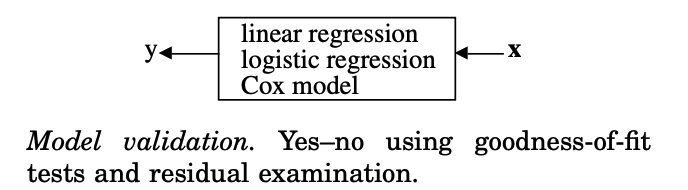
\includegraphics[width=\linewidth]{images/breiman_box1.png}
        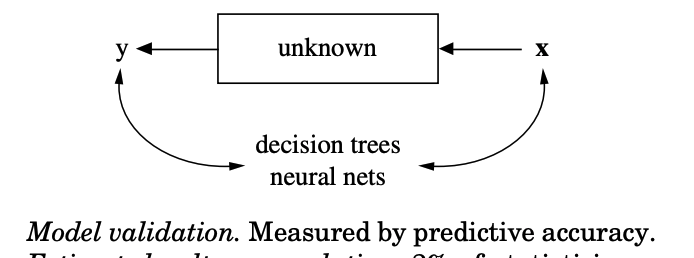
\includegraphics[width=\linewidth]{images/breiman_box2.png}        
      \end{column}%
    \end{columns}
\end{frame}


\begin{frame}{A primer on terminology}
    \begin{columns}[onlytextwidth, T] % align columns
      \begin{column}{.5\textwidth}
        \begin{wideitemize}
        \item One costly barrier to ML methods is a different terms for things
        \item Other terms worth knowing:
          \begin{itemize}
          \item ``one-hot encoding'': making dummy variables
          \item ``validation'': testing out of sample
          \end{itemize}
        \end{wideitemize}
      \end{column}%
      \hfill%
      \begin{column}{.5\textwidth}
        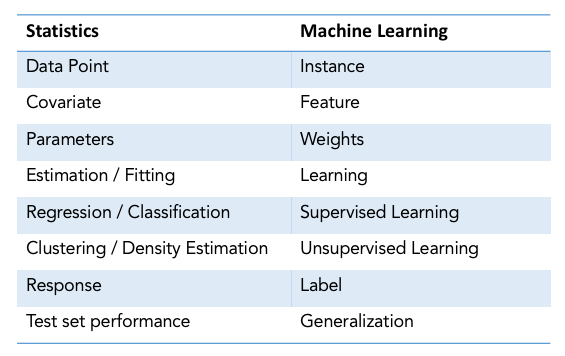
\includegraphics[width=\linewidth]{images/terminology_1.png}
        Source: ``Towards Data Science''
      \end{column}%
    \end{columns}
\end{frame}

\begin{frame}{Distinctive Features: scalability + ensemble methods}
  \begin{wideitemize}
  \item Many solution concepts for ML focus on the ability to
    \begin{enumerate}
    \item Parallelize
    \item Split data up
    \item Recombine
    \end{enumerate}
  \item The parallization has obvious reasons: computational benefits
  \item Splitting the data up is less obvious, but pivots off of a
    notion of \emph{averaging}
    \begin{itemize}
    \item Effectively, randomly smaller samples (and random subsamples
      of features) will give a noisier estimate of the ``truth''
    \item However, averaging over many of these noisy estimates will
      quickly get at the right value
    \end{itemize}
  \end{wideitemize}
\end{frame}

\begin{frame}{Distinctive Features: Testing out of sample and cross-validation}
  \begin{wideitemize}
  \item One big difference (although perhaps should not be) in ML is
    the use of out of sample testing to validate models
    \begin{itemize}
    \item This matters a ton for ML models where there is subtantial overfitting in-sample
    \end{itemize}
  \item Conceptually, consider a fully saturated model with many
    categorical variables on the right hand side:
    $$Y_{i} = X_{i}\beta + \epsilon_{i}$$
    \begin{itemize}
    \item $\beta$ is the sample mean within each $X_{i}$ bin
    \item as $dim(X_{i})$ grows relative to $n$, each bin more closely
      approximates exactly one observation
    \item This will fit \emph{very} well in-sample
      \begin{itemize}
      \item It will be quite bad out of sample!
      \end{itemize}
    \end{itemize}
  \end{wideitemize}
\end{frame}

\begin{frame}{Distinctive Features: Testing out of sample and cross-validation}
  \begin{wideitemize}
  \item Useful terminology: a training dataset, and a test dataset
    \begin{itemize}
    \item Training: estimate the model
    \item Test: evaluate the fitted model
    \end{itemize}
  \item You can easily split a sample in this way by randomizing across observations
    \begin{itemize}
    \item A crucial assumption here is independence of the observations (instances)
    \item What if they're not independent? (particularly notable in asset pricing)
      \begin{itemize}
      \item Can consider randomizing in blocks
      \item Useful to have a theory that guides these decisions
      \end{itemize}
    \end{itemize}
  \end{wideitemize}
\end{frame}



\begin{frame}{What is supervised learning / ML?}
  \begin{wideitemize}
  \item In essence, we are interested in $f(X) = E(Y | X)$
    \begin{itemize}
    \item This is exactly the same problem as our non-parametric regression question!
    \item However, in that setting, I told you to give up as soon as $dim(X)$ got large because of data issues
      \begin{itemize}
      \item ML folks are not so easily dissuaded!
      \end{itemize}
    \end{itemize}
  \item The solutions in ML revolve around different ways to circumvent a lack of data in higher dimensions
    \begin{itemize}
    \item LASSO did this using penalized methods on global (linear) functions
    \item Tree methods (next) do this by ``widening'' the comparable group
    \item Deep learning-style methods ``reduce'' the dimensionality to improve comparability
    \end{itemize}
  \end{wideitemize}
\end{frame}

\begin{frame}{Regression vs. Categorization}
    \begin{columns}[onlytextwidth, T] % align columns
      \begin{column}{.5\textwidth}
  \begin{wideitemize}
  \item Notably, ML methods distinguish between
    \begin{itemize}
    \item continuous regression problems (e.g. price as an outcome)
    \item classification problems (e.g. sold vs. not sold, or \{red bus, blue bus, car\})
    \end{itemize}
  \item In classification problems, the object is \emph{not}
    necessarily to get the probability of an event (although this is doable)
    \begin{itemize}
    \item The canonical example is digit recognition -- the USPS needs
      to identify handwritten addresses
    \item It doesn't care about an accurate measure of probabilities
      for each digit!
    \end{itemize}
  \end{wideitemize}
      \end{column}%
      \hfill%
      \begin{column}{.5\textwidth}
        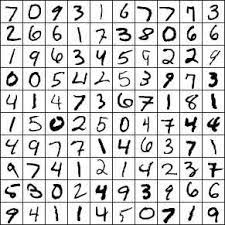
\includegraphics[width=\linewidth]{images/digits_1.jpeg}
      \end{column}%
    \end{columns}
\end{frame}

\begin{frame}{A brief tour through Trees and Forests}
  \begin{wideitemize}
  \item A very popular off-the-shelf ML model that does both regression and classification is known as regression trees
    \begin{itemize}
    \item  Combinations of trees are called forests
    \end{itemize}
  \item Given a set of parameter $X_{i}$ with $dim(X) = k$, the goal
    is to take subsets of parameters, and split the sample based on values of individual covariates $X_{ik}$
  \item The choice of split is made to minimize within-sample error within each split sample
    \begin{itemize}
    \item These splits are called ``leaves''

    \end{itemize}
  \item If we allowed infinite leaves, then the tree would grow until every observation was uniquely fit
    \begin{itemize}
    \item The solution is to penalize the number of leaves allowed via ``pruning''
    \end{itemize}
  \end{wideitemize}
\end{frame}

\begin{frame}{Trees and Forests}
  \begin{columns}[onlytextwidth, T] % align columns
    \begin{column}{.4\textwidth}
      \begin{wideitemize}
      \item In essence this approach is like exhaustively dummying but:
        \begin{itemize}
        \item The cutpoints are chosen through the data
        \item the interactions and cuts are penalized to avoid full
          saturation
        \end{itemize}
      \item These models MASSIVELY overfit in sample, however, and so
        it is important to test out of sample!
      \end{wideitemize}
      \end{column}%
      \hfill%
      \begin{column}{.6\textwidth}
        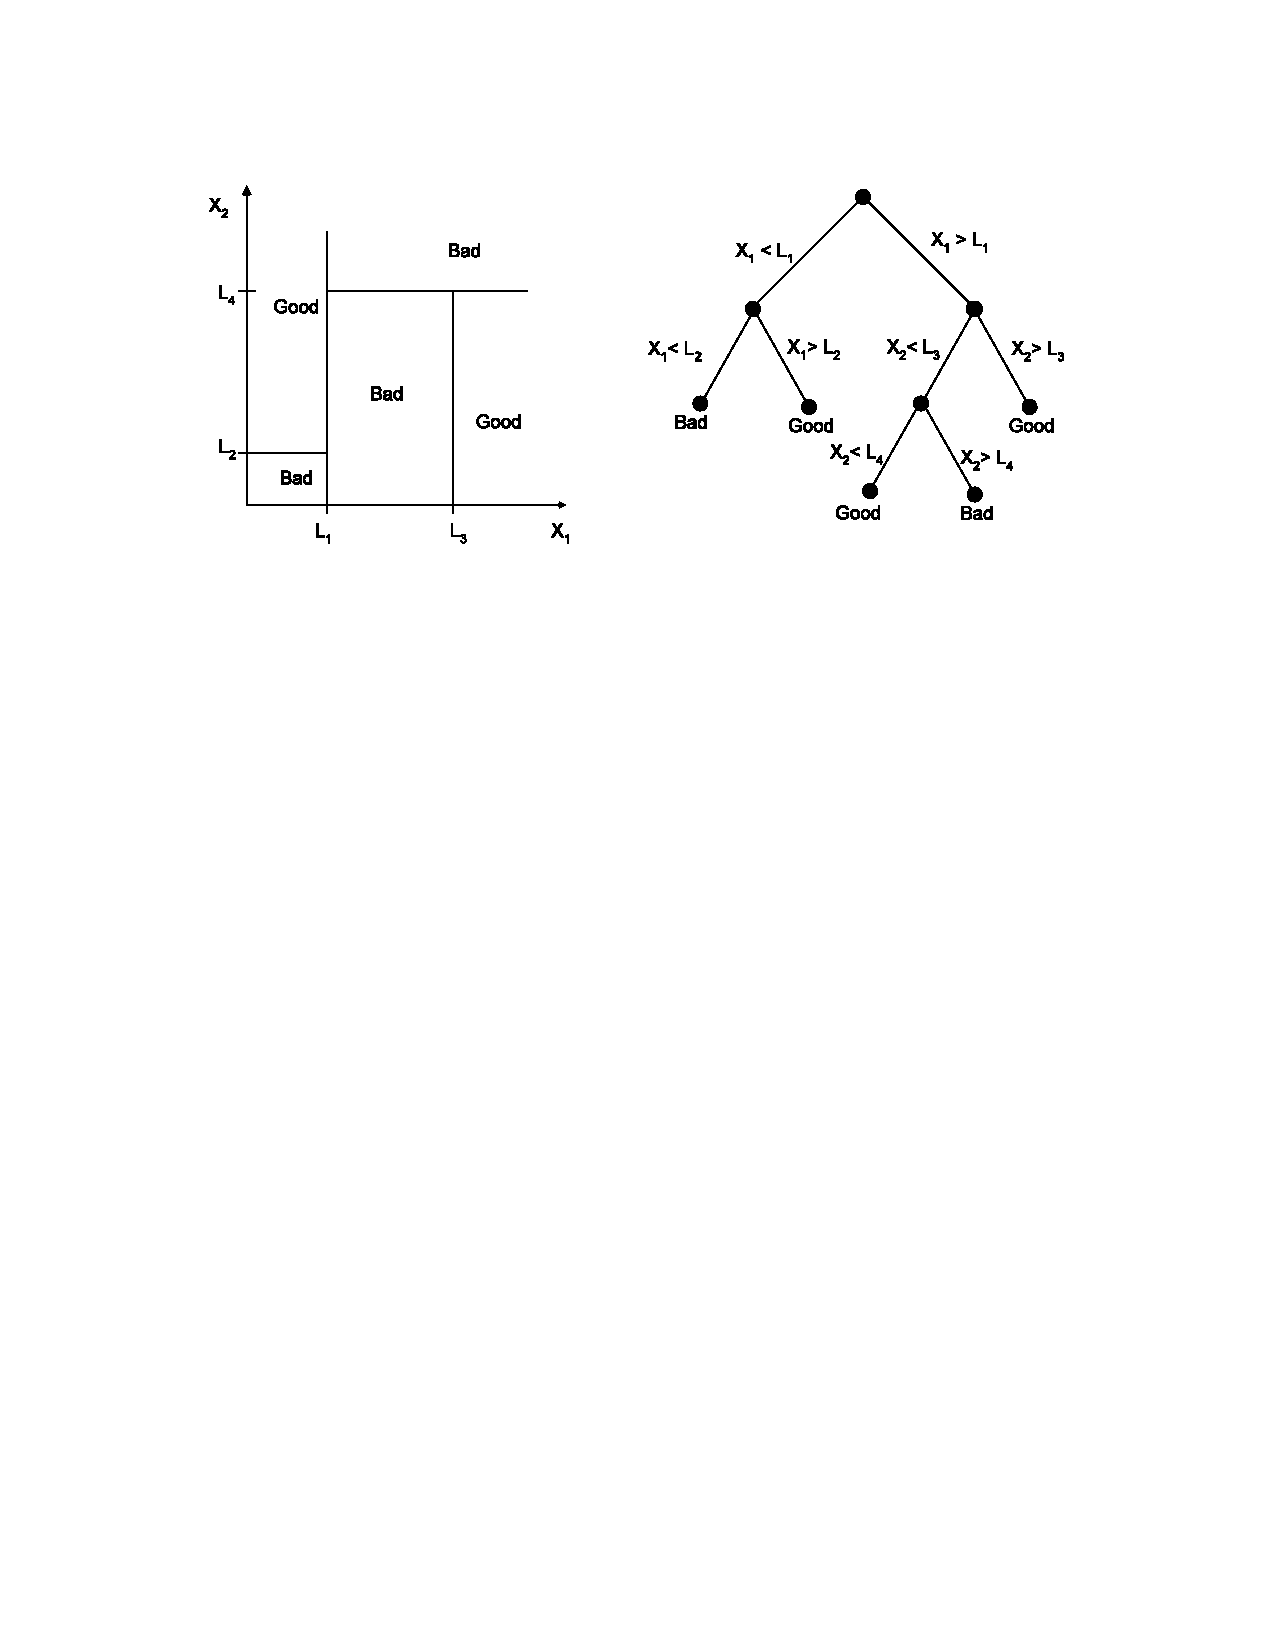
\includegraphics[width=\linewidth]{images/Tree_Lo.pdf}
      \end{column}%
    \end{columns}
\end{frame}

\begin{frame}{A brief tour through Trees and Forests}
  \begin{wideitemize}
  \item These tree models are quite discrete in their cutpoints, which can have weird properties
  \item The traditional fix to this uses \emph{Random Forests}.
  \item The approach makes many different trees to construct
    predictions, and then ``averages'' them. These trees differ in two ways:
    \begin{itemize}
    \item They use random subsamples of the data
    \item They use random subsamples of the covariates
    \end{itemize}
  \item Random sampling creates independent variation across the predictions
    \begin{itemize}
    \item Once averaged together, the overall predictions are quite a
      bit smoother and also better fit out of sample
    \end{itemize}
  \end{wideitemize}
\end{frame}

\begin{frame}{An example Forest}
  \begin{columns}[onlytextwidth, T] % align columns
    \begin{column}{.4\textwidth}
      \begin{wideitemize}
      \item These models can create much more non-linear relationships
        than say, Logit
      \item Example from Fuster et al. (2021)
      \end{wideitemize}
      \end{column}%
      \hfill%
      \begin{column}{.6\textwidth}
        \only<1>{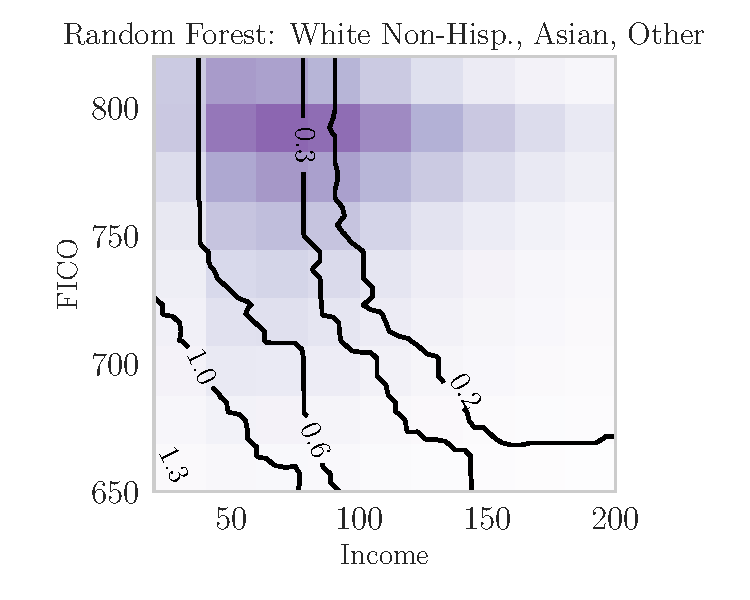
\includegraphics[width=\linewidth]{images/pd_dist_contour_1_1.pdf}}
        \only<2>{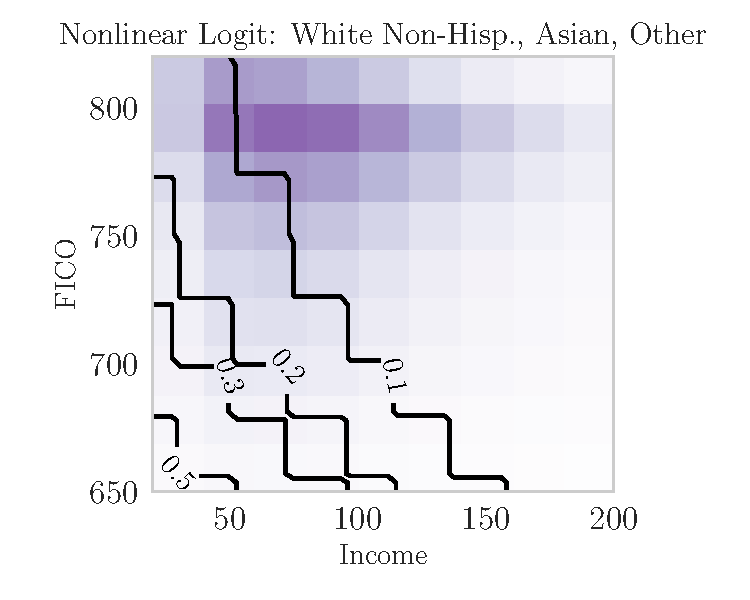
\includegraphics[width=\linewidth]{images/pd_dist_contour_0_1.pdf}}        
      \end{column}%
    \end{columns}
\end{frame}

\begin{frame}{Three key insights from ML (Breiman (2001))}
  \begin{columns}[onlytextwidth, T] % align columns
    \begin{column}{.5\textwidth}
  \begin{wideitemize}
  \item<1-> Once you are fitting to predict outcome as accurately as
    possible, there are potentially many equally good models that will put weight on different inputs
    (\textbf{Rashomon})
  \item<2-> Simple and transparent models tend to be less accurate (\textbf{Occam})
  \item<3-> Dimensionality is a \emph{benefit} in ML (unlike traditional non-parametrics) (\textbf{Bellman})
  \end{wideitemize}
      \end{column}%
      \hfill%
      \begin{column}{.4\textwidth}
        \only<1>{
\includegraphics[width=\linewidth]{images/rashomon.jpeg}}
        \only<2>{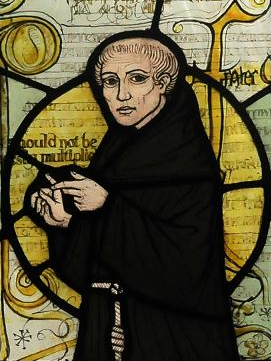
\includegraphics[width=\linewidth]{images/occam.png}}
        \only<3>{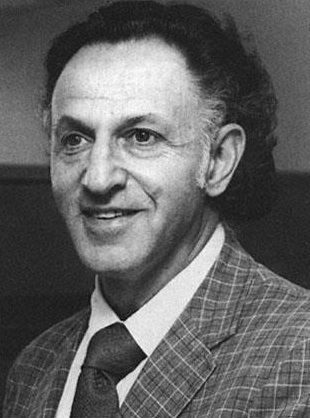
\includegraphics[width=\linewidth]{images/bellman.jpg}}        
      \end{column}%
    \end{columns}
\end{frame}

\begin{frame}{Implications of Rashomon}
  \begin{wideitemize}
  \item Formally,
    \begin{quote} What I call the Rashomon Effect is
      that there is often a multitude of different descriptions
      [equations fx] in a class of functions giving about the same
      minimum error rate.
    \end{quote}
  \item One important implication of this is model averaging can be
    very successful, since the paths to getting similar error rates
    can be independent (``bagging'')
  \item \emph{significantly} cautions interpretation of weights from
    model inputs
  \item Also means that models may be highly sensitive!
  \end{wideitemize}
\end{frame}

\begin{frame}{Implications of Rashomon (D'amour (2021))} 
  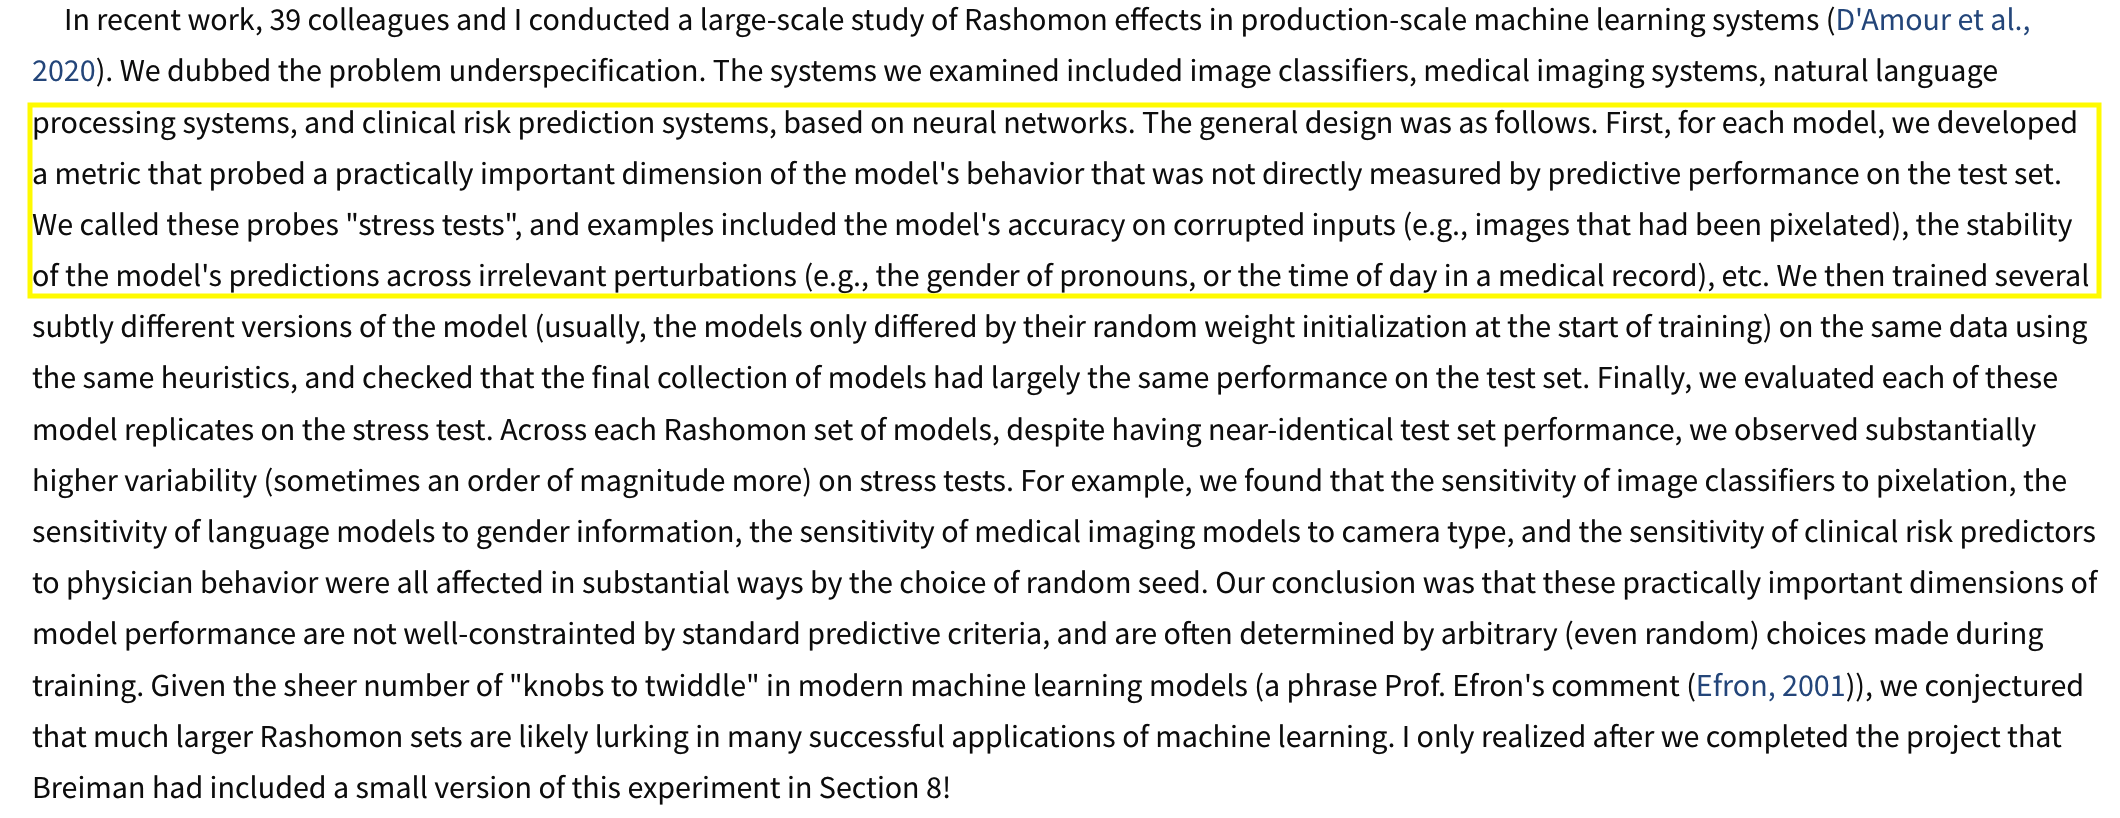
\includegraphics[width=0.8\linewidth]{images/rashomon_stresstest.png}
\end{frame}

\begin{frame}{Implications of Occam}
  \begin{wideitemize}
  \item Many of the most effective models are hard to ``explain''
    \begin{itemize}
    \item e.g., what drives the Random Forest model?
    \end{itemize}
  \item Is there a given input that matters? In OLS, we can look at coefficients
  \item This is a serious challenge in ML models (especially once
    combined with Rashomon)
    \begin{itemize}
    \item Better to use ML to substitiute for ``nuisance'' parameters
    \end{itemize}
  \end{wideitemize}
\end{frame}


\begin{frame}{Implications of Bellman}
  \begin{wideitemize}
  \item Recall that for a fixed sample $n$, if we increase the number
    of features (covariates) $K$, we will get noisier and noisier
    estimates with something like OLS (or non-parametric estimation)
  \item This is what Richard Bellman termed ``the curse of dimensionality''
  \item This curse is a blessing for many ML applications; why?
    \begin{itemize}
    \item The curse shows up in estiamting underlying parameters
    \item When focusing on the outcome, $y$, the solutions often
      improve as you increase the dimensionality
    \item This is due, implicitly, to penalization, and avoiding a
      focus on unbiasedness
    \end{itemize}
  \item Hence, key insight: rather than throw out data, use shrinkage
    (via penalization, or priors) to maintain an effective prediction
    \begin{itemize}
    \item This insight goes back to Stein (1956)!
    \end{itemize}
  \end{wideitemize}
\end{frame}


\begin{frame}{The virtue of complexity (and the double descent)}
  \begin{wideitemize}
  \item As models grow in complexity, 
  \begin{itemize}
    \item there is a decrease in the ``in-sample'' error that continues until you have a fully saturated model
    \item there is an initial decrease in the ``out-of-sample'' error initially, and then an increase due to overfitting
  \end{itemize}
  \item This trade-off is what is often optimized using cross-validation
  \item However, a key new insight (see Kelly, Malamud and Zhou (2024) for an example) is that the out-of-sample error will start to improve again as the number of parameters grows (under certain models)
  \item This is the ``double descent'' curve
  \begin{itemize}
    \item Big improvements in predicting future market returns (market timing)
    \item Interesting to think of applications in other areas!
  \end{itemize}
  \end{wideitemize}
\end{frame}

\begin{frame}
  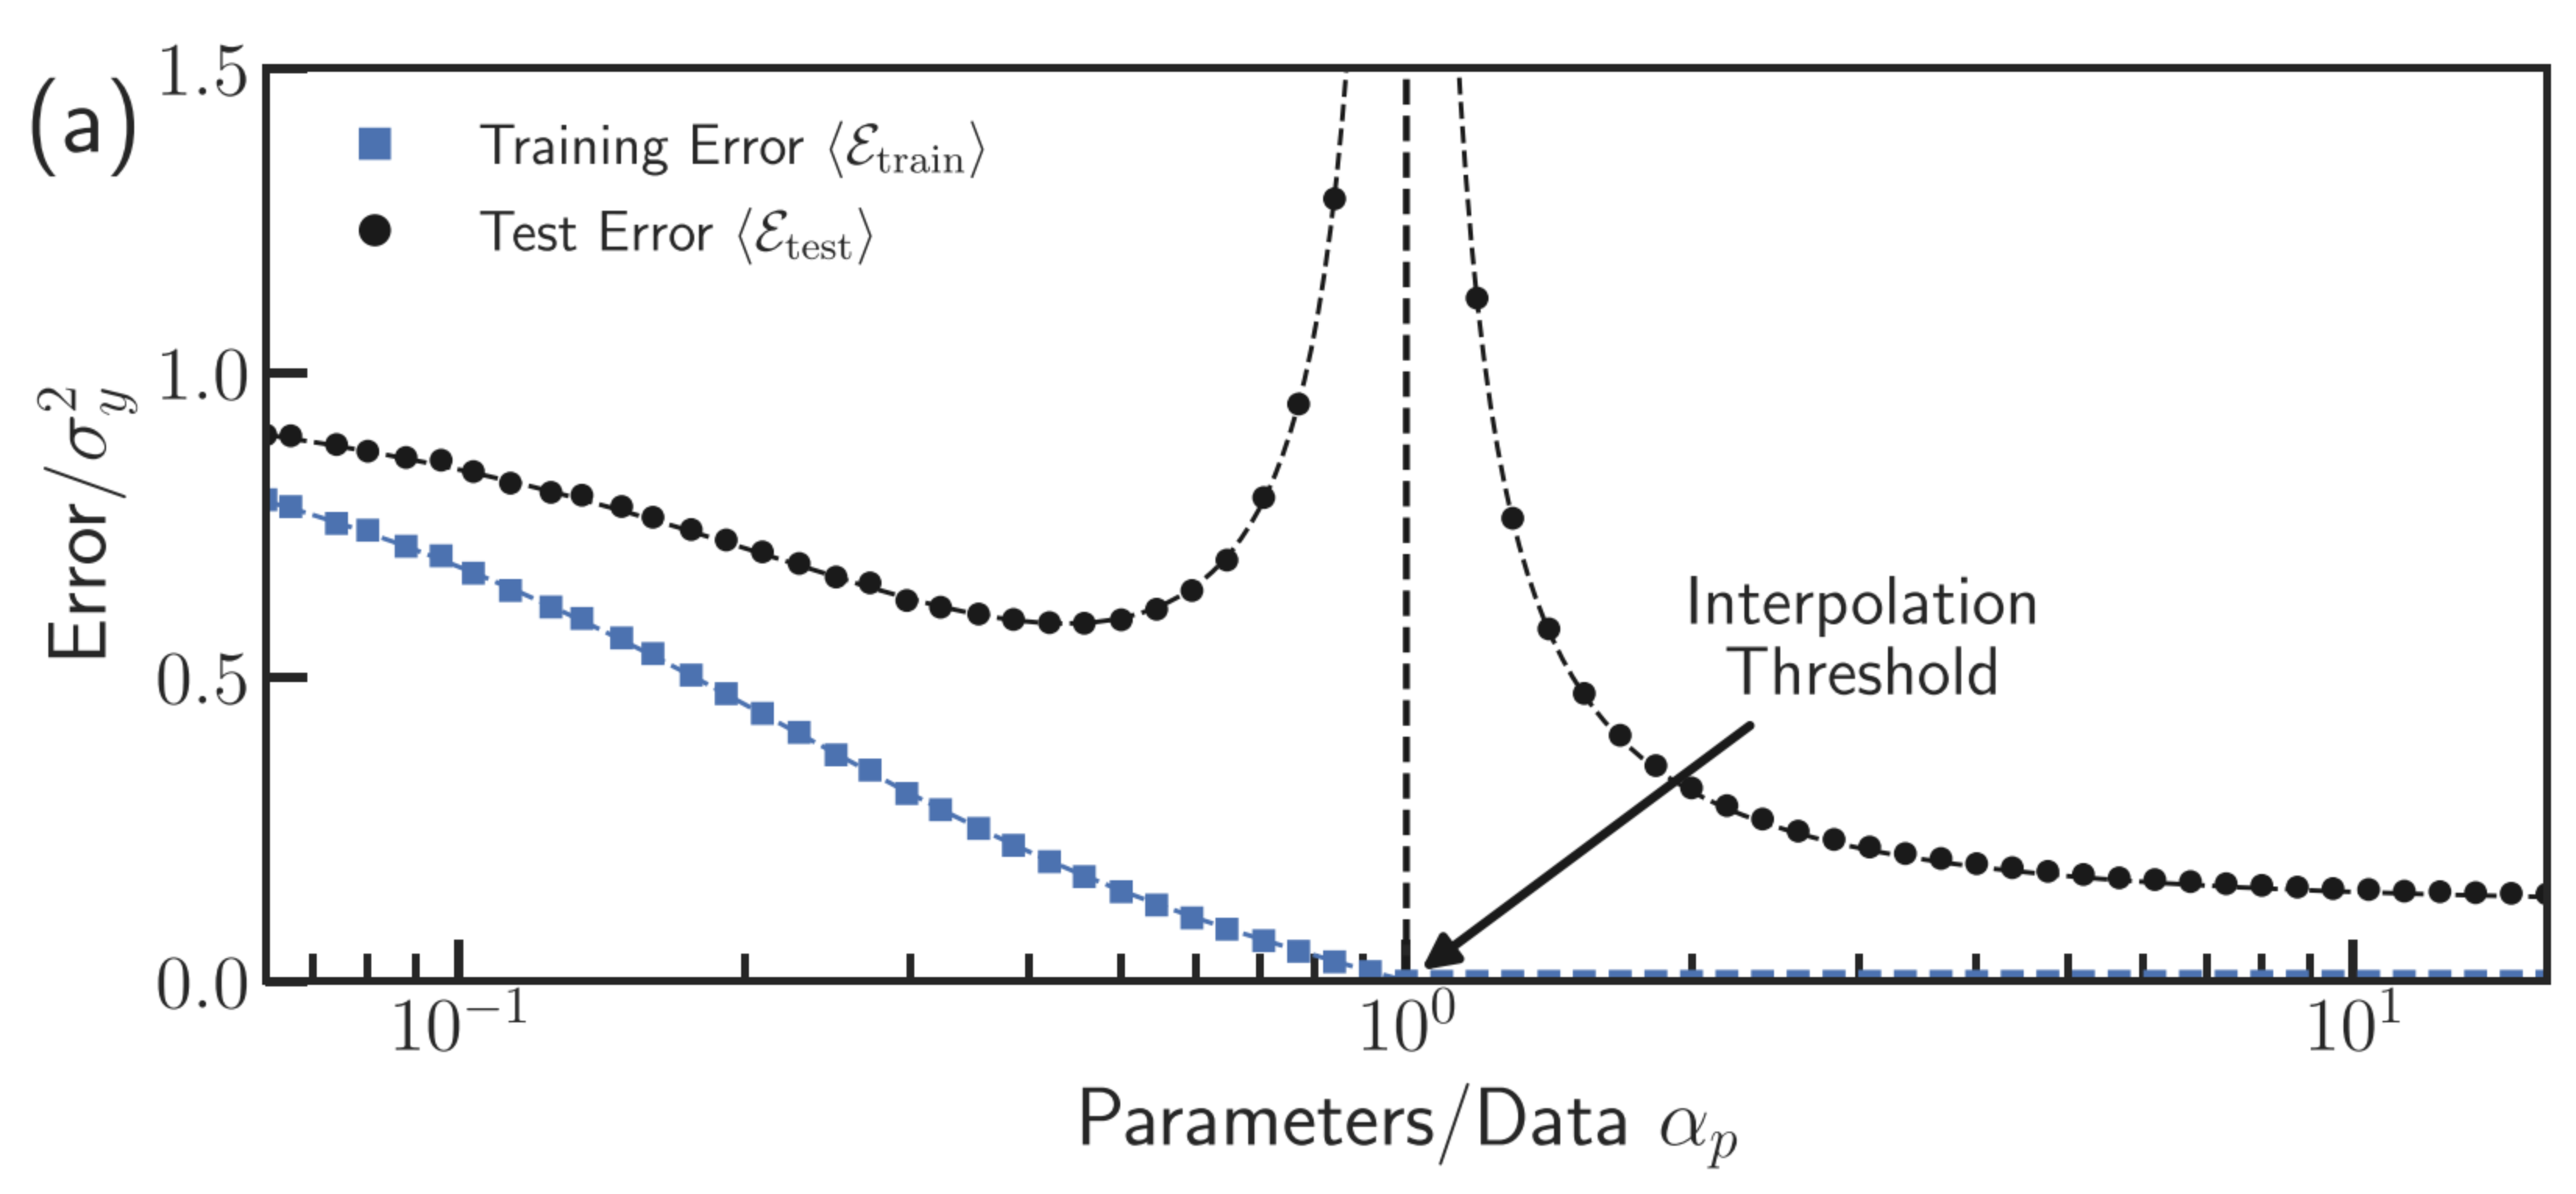
\includegraphics[width=\linewidth]{images/double_descent.png}
\end{frame}





\begin{frame}{How to approach and further reading}
  \begin{wideitemize}
  \item If you are considering ML models, the two standard programming
    languages with significant support are Python and R
    \begin{itemize}
    \item It's possible that Julia and Matlab are doable, but I have seen far less here
    \end{itemize}
  \item In Python, \texttt{scikit-learn} is a great package with many features
  \item In R, there is a big community of a packages that can be used
    as well, with \texttt{caret} as a very useful meta-engine for
    running diffferent estimations
    \begin{itemize}
    \item ``Hands-On Machine Learning in R'' is an excellent resource
      for this: \url{https://bradleyboehmke.github.io/HOML/}
    \end{itemize}
  \item The biggest challenge in my experience, is that the high-level
    concepts are very straightforward, while the nitty-gritty tuning,
    testing and decipering is quite hard
    \begin{itemize}
    \item A big reason this is true is that it's very application-specific
    \item Different forecasting problems have different issues
    \end{itemize}
  \end{wideitemize}
\end{frame}

\begin{frame}{Checklist for what to look for}
  \begin{wideitemize}
  \item What type of outcome do I have? (Classification vs. Regression)
  \item Do I expect highly non-linear responses, or relatively linear ones?
    \begin{itemize}
    \item Many economics models have relatively monotonic response patterns
    \item Linear models might do just fine!
    \end{itemize}
  \item Do not use these models for data exploration -- they can be
    computationally quite expensive, and are much less transparent
    \begin{itemize}
    \item Identify your prediction problem carefully, and setup your
      estimation accordingly to cross-validate on appropriate
      parameters
    \end{itemize}
  \end{wideitemize}
\end{frame}

\end{document}